\documentclass[crop,class=article]{standalone}
%----------------------------Preamble-------------------------------%
\usepackage{tikz}
\usepackage{amsmath}
\usetikzlibrary{arrows.meta}
%--------------------------Main Document----------------------------%
\begin{document}
    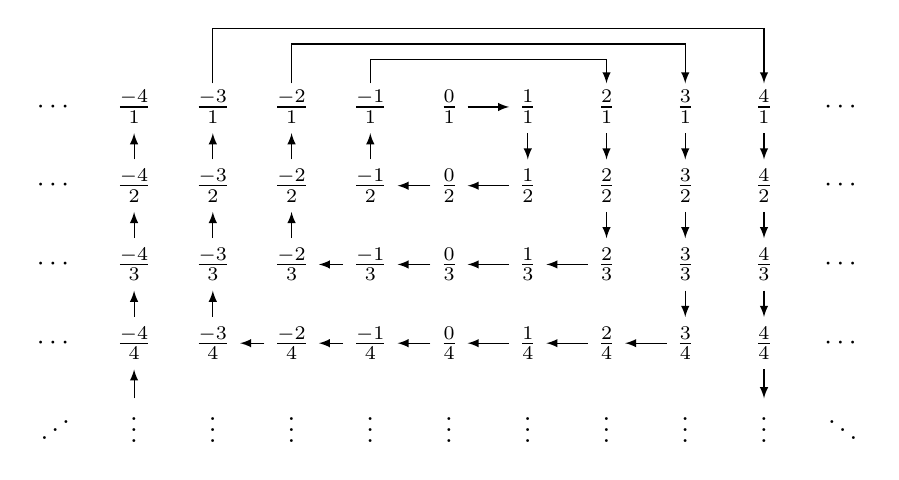
\begin{tikzpicture}[%
        >=latex
    ]
        \foreach\y in {1, 2, 3, 4}{%
            \foreach\x in {-4, -3, -2, -1, 0, 1, 2, 3, 4}{%
                \node (\x\y) at (\x, 7-\y) {$\frac{\x}{\y}$};
            }
        }
        \foreach\x in {-4, -3, -2, -1, 0, 1, 2, 3, 4}{%
            \node at (\x, 2) {$\vdots$};
        }
        \foreach\y in {3, 4, 5, 6}{%
            \node at (5, \y) {$\cdots$};
            \node at (-5, \y) {$\cdots$};
        }
        \node at (5, 2) {$\ddots$};
        \node at (-5, 2) {$\reflectbox{\ensuremath{\ddots}}$};
        \draw[->] (01) to (11);
        \draw[->] (11) to (12);
        \draw[->] (12) to (02);
        \draw[->] (02) to (-12);
        \draw[->] (-12) to (-11);
        \draw[->] (-1, 6.3) to (-1, 6.6)
                            to (2, 6.6)
                            to (2, 6.3);
        \draw[->] (21) to (22);
        \draw[->] (22) to (23);
        \draw[->] (23) to (13);
        \draw[->] (13) to (03);
        \draw[->] (03) to (-13);
        \draw[->] (-13) to (-23);
        \draw[->] (-23) to (-22);
        \draw[->] (-22) to (-21);
        \draw[->] (-2, 6.3) to (-2, 6.8)
                            to (3, 6.8)
                            to (3, 6.3);
        \draw[->] (31) to (32);
        \draw[->] (32) to (33);
        \draw[->] (33) to (34);
        \draw[->] (34) to (24);
        \draw[->] (24) to (14);
        \draw[->] (14) to (04);
        \draw[->] (04) to (-14);
        \draw[->] (-14) to (-24);
        \draw[->] (-24) to (-34);
        \draw[->] (-34) to (-33);
        \draw[->] (-33) to (-32);
        \draw[->] (-32) to (-31);
        \draw[->] (-3, 6.3) to (-3, 7)
                            to (4, 7)
                            to (4, 6.3);
        \draw[->] (41) to (42);
        \draw[->] (42) to (43);
        \draw[->] (43) to (44);
        \draw[->] (44) to (4, 2.3);
        \draw[->] (-4, 2.3) to (-44);
        \draw[->] (-44) to (-43);
        \draw[->] (-43) to (-42);
        \draw[->] (-42) to (-41);
    \end{tikzpicture}
\end{document}